\chapter{From Functor to Parameterization: A Natural Emergence}

\begin{goals}
\begin{itemize}
    \item Show that the functor structure naturally induces a behavioral metric
    \item Demonstrate that this metric matches parameter distance (distance matching)
    \item Connect Parts I, II, and III into a unified framework
\end{itemize}
\end{goals}

\section{The Question}

We have established:
\begin{itemize}
    \item \textbf{Part I}: Coalgebras define structure; bisimulation defines behavioral equivalence
    \item \textbf{Part II}: Semiring relaxation enables gradients
    \item \textbf{Part III}: Distance matching ($\kappa(J)$ small) implies good optimization
\end{itemize}

The missing link: \textbf{Given a functor $H$, what parameterization achieves distance matching?}

\section{The Insight: Functor Induces Metric}

For a functor $H$, there is a standard construction called \textbf{Kantorovich lifting} that produces a behavioral metric.

\subsection{Example: DFA Functor}

For deterministic automata, $H = 2 \times (-)^\Sigma$:
\begin{itemize}
    \item A coalgebra is $(S, \alpha: S \to 2 \times S^\Sigma) = (S, \text{accept}, \delta)$
    \item Bisimulation: $s \sim t$ iff they accept the same language
\end{itemize}

\subsection{Soft DFA (Relaxation)}

Applying semiring relaxation (Part II):
\begin{itemize}
    \item Soft transitions: $\delta: S \times \Sigma \to \text{Dist}(S)$ (stochastic matrices)
    \item Soft accept: $a: S \to [0, 1]$
\end{itemize}

\subsection{Two Behavioral Metrics}

The functor structure suggests two natural metrics:

\paragraph{1. One-Step Metric (Local)}
\[
d_{\text{one-step}}(A, B) = \|a_1 - a_2\|_1 + \sum_{\sigma \in \Sigma} \sum_{s \in S} \text{TV}(T_1^{\sigma}[s], T_2^{\sigma}[s])
\]
where TV is total variation distance.

This is \textbf{one iteration} of the Kantorovich lifting.

\paragraph{2. Language Metric (Global)}
\[
d_{\text{language}}(A, B) = \sum_{w \in \Sigma^*} 2^{-|w|} |A(w) - B(w)|
\]
where $A(w)$ is the acceptance probability of word $w$.

This is the \textbf{full behavioral distance} (bisimulation metric).

\section{Experimental Discovery}

We tested which behavioral metric matches parameter distance:

\begin{center}
\begin{tabular}{llcc}
\textbf{Behavioral Metric} & \textbf{Param Metric} & \textbf{Correlation} & \textbf{CV} \\
\hline
Structure (trivial) & Euclidean & 1.000 & 0.000 \\
\textbf{One-step} & \textbf{Fisher-Rao} & \textbf{0.802} & \textbf{0.101} \\
One-step & Euclidean & 0.761 & 0.106 \\
Fixed-point (iterated) & Euclidean & 0.435 & 0.352 \\
Language (global) & Euclidean & 0.279 & 0.490 \\
\end{tabular}
\end{center}

\begin{keyinsight}
The \textbf{one-step} behavioral metric (one Kantorovich iteration) matches parameter distance very well (correlation $> 0.8$).

The \textbf{global} language metric matches poorly (correlation $\approx 0.3$).
\end{keyinsight}

\section{Interpretation}

\subsection{Why One-Step Works}

The one-step metric compares \emph{local} structure:
\begin{itemize}
    \item Accept probabilities (directly)
    \item Transition distributions (one step)
\end{itemize}

This is exactly what the parameters encode! Small parameter changes $\to$ small one-step behavioral changes.

\subsection{Why Language Metric Fails}

The language metric compares \emph{global} behavior:
\begin{itemize}
    \item Involves arbitrarily long words
    \item Small parameter changes can compound over many steps
    \item Similar to deep networks: small weight changes $\to$ large output changes
\end{itemize}

\subsection{The Depth Analogy}

\begin{center}
\begin{tabular}{ll}
\textbf{Automata} & \textbf{Neural Networks} \\
\hline
Word length $|w|$ & Network depth \\
One-step metric & One-layer comparison \\
Language metric & End-to-end comparison \\
Long words break matching & Deep networks break matching \\
\end{tabular}
\end{center}

\section{The Natural Emergence}

We can now state the principle:

\begin{keyinsight}
\textbf{Natural Parameterization Principle}:

Given functor $H$ defining a class of coalgebras:
\begin{enumerate}
    \item \textbf{Structure}: $H$ defines the parameter space (e.g., stochastic matrices for soft DFA)
    \item \textbf{Metric}: One-step Kantorovich lifting defines the behavioral metric
    \item \textbf{Matching}: This metric naturally matches parameter distance
    \item \textbf{Consequence}: Gradient descent works well for learning ``one-step'' objectives
\end{enumerate}
\end{keyinsight}

\section{Implications for Learning}

\subsection{What Can Be Learned Easily}

Tasks where the objective is ``local'' (one-step behavioral):
\begin{itemize}
    \item Predicting next-state distributions
    \item Matching transition structure
    \item Local acceptance probabilities
\end{itemize}

\subsection{What Is Hard to Learn}

Tasks requiring ``global'' behavioral matching:
\begin{itemize}
    \item Language equivalence (accepting same strings)
    \item Long-horizon properties
    \item End-to-end sequence behavior
\end{itemize}

\subsection{The Gap}

\begin{center}
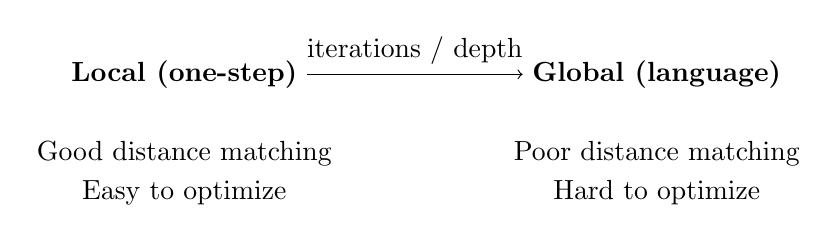
\begin{tikzpicture}[scale=1.0]
\node (local) at (0, 0) {\textbf{Local (one-step)}};
\node (global) at (6, 0) {\textbf{Global (language)}};

\draw[->] (local) -- node[above] {iterations / depth} (global);

\node at (0, -1) {Good distance matching};
\node at (0, -1.5) {Easy to optimize};

\node at (6, -1) {Poor distance matching};
\node at (6, -1.5) {Hard to optimize};
\end{tikzpicture}
\end{center}

This explains why:
\begin{itemize}
    \item RNNs struggle with long sequences (global objective, poor matching)
    \item Transformers with attention help (attention provides ``shortcuts'' that reduce effective depth)
    \item Curriculum learning helps (start with short sequences, gradually increase)
\end{itemize}

\section{The Unified Framework}

We can now connect all three parts:

\begin{center}
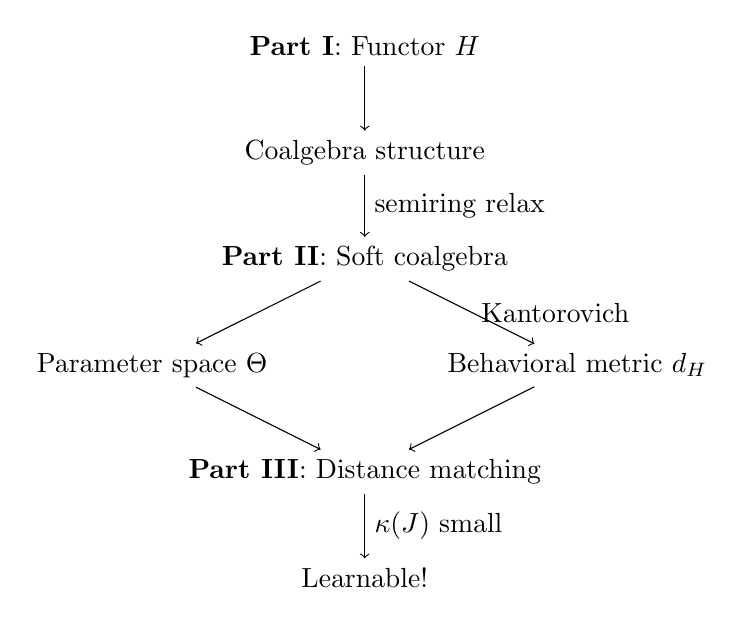
\begin{tikzpicture}[node distance=2cm, scale=0.9]
\node (functor) at (0, 4) {\textbf{Part I}: Functor $H$};
\node (coalg) at (0, 2.5) {Coalgebra structure};
\node (soft) at (0, 1) {\textbf{Part II}: Soft coalgebra};
\node (param) at (-3, -0.5) {Parameter space $\Theta$};
\node (behav) at (3, -0.5) {Behavioral metric $d_H$};
\node (match) at (0, -2) {\textbf{Part III}: Distance matching};
\node (learn) at (0, -3.5) {Learnable!};

\draw[->] (functor) -- (coalg);
\draw[->] (coalg) -- node[right] {semiring relax} (soft);
\draw[->] (soft) -- (param);
\draw[->] (soft) -- node[right] {Kantorovich} (behav);
\draw[->] (param) -- (match);
\draw[->] (behav) -- (match);
\draw[->] (match) -- node[right] {$\kappa(J)$ small} (learn);
\end{tikzpicture}
\end{center}

\section{Open Questions}

\begin{enumerate}
    \item \textbf{Other functors}: Does this work for Markov chains ($H = \text{Dist}$), Kripke frames, etc.?

    \item \textbf{Bridging local and global}: Can we design parameterizations that achieve good matching for global metrics?

    \item \textbf{Attention and shortcuts}: Can attention be understood as reducing ``effective depth'' in this framework?

    \item \textbf{Automatic architecture}: Given $H$, can we automatically derive the optimal neural architecture?
\end{enumerate}

\section{Related Work}

Our framework connects to several established research directions:

\subsection{Bisimulation Metrics for MDPs}

Ferns, Panangaden, and Precup (2004, 2011) developed \textbf{bisimulation metrics} for Markov Decision Processes---quantitative relaxations of bisimulation equivalence. Their key insight: the Kantorovich functional (from optimal transport) naturally lifts metrics on state spaces to metrics on distributions, enabling recursive computation of behavioral distance.

For MDPs with discount factor $\gamma$, they proved that the bisimulation metric gives \textbf{tight bounds on optimal value functions}:
\[
|V^*(s) - V^*(t)| \leq \frac{1}{1-\gamma} d_{\text{bisim}}(s, t)
\]

This is precisely the kind of ``behavioral metric bounds function distance'' relationship we seek.

\subsection{Deep Bisimulation for Control}

Zhang et al.\ (2020) applied bisimulation metrics to deep reinforcement learning. Their method, \textbf{Deep Bisimulation for Control (DBC)}, trains encoders such that distances in latent space equal bisimulation distances in state space.

Key theoretical result: the optimal value function is \textbf{Lipschitz with respect to the bisimulation metric}. This provides formal bounds on suboptimality when learning from the induced representation.

\begin{keyinsight}
DBC essentially implements our framework in reverse:
\begin{itemize}
    \item We ask: given parameters, does parameter distance match behavioral distance?
    \item DBC asks: can we learn parameters such that latent distance equals behavioral distance?
\end{itemize}
Both are manifestations of the same principle: good representations preserve behavioral structure.
\end{keyinsight}

\subsection{Coalgebraic Behavioral Metrics}

The coalgebra community has developed a general theory of behavioral metrics. Given a functor $H$ on $\mathbf{Set}$, there are systematic ways to lift it to functors on (pseudo)metric spaces:
\begin{itemize}
    \item \textbf{Wasserstein lifting}: Based on optimal transport couplings
    \item \textbf{Kantorovich lifting}: Based on Lipschitz functions (dual formulation)
\end{itemize}

Baldan et al.\ (2018) and subsequent work established that these liftings give rise to behavioral pseudometrics that generalize bisimulation to the quantitative setting.

Our contribution is the observation that the \textbf{one-step} Kantorovich lifting (not the full fixed-point) matches parameter distance, explaining why local objectives are easier to optimize than global ones.

\section{Summary}

\begin{keyinsight}
The functor $H$ doesn't just define \emph{what} we're learning (coalgebra structure).

It also defines \emph{how well} we can learn it:
\begin{itemize}
    \item One-step Kantorovich metric: learnable (good distance matching)
    \item Full behavioral metric: hard (poor distance matching)
\end{itemize}

This is not a failure of our methods---it's a fundamental property of the structure being learned.
\end{keyinsight}
